\documentclass[tikz, border=1mm]{standalone}
\begin{document}
	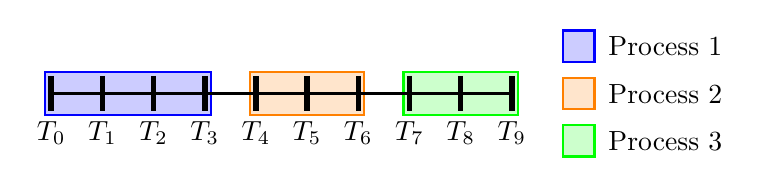
\begin{tikzpicture}
	\def \m {1.3}		
	\draw[draw=blue, thick, fill=blue!20] (0*\m-0.075,0.275) rectangle (1.5*\m+0.075,-.275);
	\draw[draw=orange, thick, fill=orange!20] (2*\m-0.075,0.275) rectangle (3*\m+0.075,-.275);
	\draw[draw=green, thick, fill=green!20] (3.5*\m-0.075,0.275) rectangle (4.5*\m+0.075,-.275);

	\draw[draw=blue, thick, fill=blue!20] (5*\m,0.8) rectangle (5*\m+0.4,.4);
	\draw[draw=orange, thick, fill=orange!20] (5*\m,0.2) rectangle (5*\m+0.4,-.2);
	\draw[draw=green, thick, fill=green!20] (5*\m,-0.4) rectangle (5*\m+0.4,-.8);

	\draw (5*\m+1.3,.6) node {Process 1};
	\draw (5*\m+1.3,.0) node {Process 2};
	\draw (5*\m+1.3,-.6) node {Process 3};
	


	\draw[line width=1.2pt] (0*\m,0) -- (4.5*\m,0);
	\foreach \i in {0,.5,1,...,4.5}{
		\draw[line width=2pt] (\i*\m,.225) -- (\i*\m,-.225);
	}
	
	\draw (0.0*\m,-.5) node {$T_0$};
	\draw (0.5*\m,-.5) node {$T_1$};
	\draw (1.0*\m,-.5) node {$T_2$};
	\draw (1.5*\m,-.5) node {$T_3$};
	\draw (2.0*\m,-.5) node {$T_4$};
	\draw (2.5*\m,-.5) node {$T_5$};
	\draw (3.0*\m,-.5) node {$T_6$};
	\draw (3.5*\m,-.5) node {$T_7$};
	\draw (4.0*\m,-.5) node {$T_8$};
	\draw (4.5*\m,-.5) node {$T_9$};

		
	\end{tikzpicture}
\end{document}